\chapter{Charakterystyka ruchu pieszych}
\label{cha:charakterystykaRuchu}

\section{Points of interest}
\label{sec:pointsOfInterest}

Pieszy nigdy nie porusza się tylko i wyłącznie z punktu A do punktu B. Często po drodze zatrzymujemy się w sklepie czy oglądam reklamy. Biorąc pod uwagę takie zachowania wyróżnione zostały punkty POI (\textit{ang. Points of intrests}). Agent może dokonać wyboru danego punktu (bądź nie) po czym jego aktualny stan zmienia się odpowiednio z ruchu na stan oczekiwania lub odwrotnie. Wprowadzenie takiej zależności pozwala zaimplementować ruch bardziej realistycznie. Przy POI wzrasta gęstość tłumu, przez ścieżki ruchu innych uczestników ruchu ulegają zmianie.
 
\section{Strefa prywatna}
\label{sec:strefaPryw}

Dla każdego pieszego definiuje się opisaną wcześniej strefę prywatną. Im bliżej przeszkody lub innego agenta, tym pieszy czuje się mniej komfortowo i utrzymuje dystans od sąsiada, zależny od konkretnej sytuacji. Strefa prywatna pomaga unikać kolizji w przypadkach nagłej zmiany prędkości przez innych uczestników ruchu.

\section{Czas relaksacji}
\label{sec:czasRelaksacji}

Piesi zmieniając kierunek swojej drogi potrzebują pewną (niewielką) ilość czasu na podjęcie decyzji. Z tego względu we wzorze został wprowadzony \textit{czas relaksacji}. Wartość przyjęta w~symulacji to $0.5 sek$

\section{Czekający piesi}
\label{sec:czekajacyPiesi}

Czekający piesi są częstymi uczestnikami normalnego ruchu. Czekający piesi mogą powodować korki \cite{6}. Modelowanie czekających pieszych ma dwa aspekty: reakcje  przechodzących obok pieszych na pozostającego w spoczynku oraz pozostającego w spoczynku na poruszających się.

\section{Formowanie strug}
\label{sec:strugi}

Bazując na pracy \cite{HeBuAjTw} zakłada się, że piesi preferują ruch za innym z pieszych. W szczególności taki zachowanie może zostać zaobserwowane, kiedy die strugi pieszych przemieszczają się w przeciwnych kierunkach. Jest to spowodowane mniejszymi interakcjami z innymi uczestnikami ruchu oraz tym, że przerwanie strugi pieszych zdarza się stosunkowo rzadko.

\begin{figure}
\centering
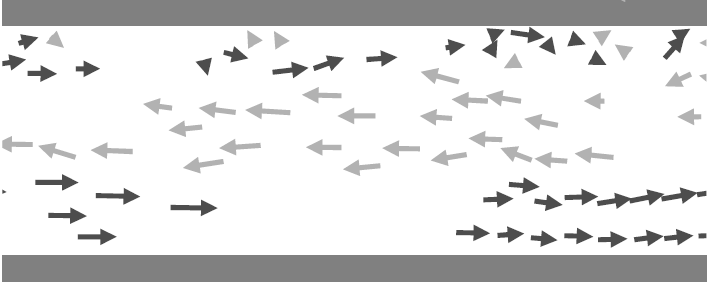
\includegraphics[width=0.7\textwidth]{line.png}
\caption{Formowanie strug, opracowanie \cite{HeBuAjTw}}
\end{figure}

\section{Unikanie kolizji}
\label{sec:kolizje}

Podczas każdej zmiany położenia podczas symulacji należy upewnić się czy po przejściu nie dojdzie do kolizji z innymi uczestnikami ruchu czy przeszkodami. W~przypadku kolizji należy sprawdzić jej typ i~dostosować do niej zachowanie jednostki. Do kolizji może dość w~przypadku, kiedy dwoje pieszych~w następnym kroku mają przejść na to samo miejsce lub kiedy zamieniają się miejscami. Każda~z kolizji wymaga podjęcia innych kroków, aby jej uniknąć. Po uniknięciu kolizji pieszy powinien powrócić do swojej pierwotnej ścieżki ruchu. Każdy z~pieszych ma także pewien priorytet zależny od takich cech jak niepełnosprawność itp. Zgodnie z pracą Charif Foudil \cite{Collision} możemy wyróżnić trzy typy kolizji.

\subsection{Kolizja czołowa}

Występuje w przypadku, kiedy dwoje pieszych idzie prosto na siebie. Na samym początku należy określić, czy piesi kolidują ze sobą po lewej czy po prawej stronie (rzadko zdarza się ruch dokładnie na wprost siebie). Piesi preferują takie uniknięcie kolizji, jakie pozwoli im na jak najmniejsze odchylenie od ich wyznaczonej wcześniej trasy. Możemy wyróżnić trzy możliwości uniknięcia takiej kolizji:

\begin{itemize}
\item zmianę kierunku ruchu
\item zmianę prędkości
\item zmianę zarówno kierunku, jak i prędkości
\end{itemize}

Jeśli żaden ze sposobów nie zadziała, pieszy zatrzyma się, przepuszczając drugiego uczestnika ruchu, a następnie ruszy wyznaczoną wcześniej trasą.


\begin{figure}
\centering
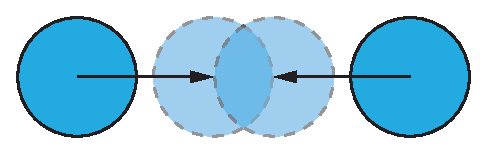
\includegraphics[width=0.4\textwidth]{kolizjaczolowa.eps}
\caption{Schemat kolizji czołowej, opracowanie własne}
\end{figure}

\subsection{Kolizja boczna}

Kolizja, której rozwiązanie jest podobne jak dla \textit{kolizji czołowej}.

\begin{figure}
\centering
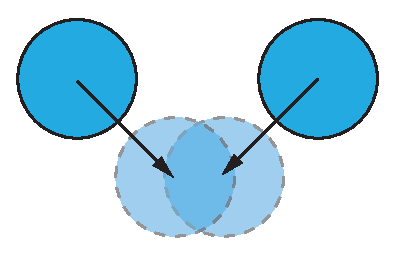
\includegraphics[width=0.4\textwidth]{kolizjaboczna.eps}
\caption{Schemat kolizji czołowej, opracowanie własne}
\end{figure}

\subsection{Kolizja tylna}

Ma miejsc, gdy pieszy porusza się z większą prędkością niż inny uczestnik ruchu pokonujący przed nim tę samą drogę. W tym przypadku pieszy o większej prędkości może:

\begin{itemize}
\item zwolnić do takiej samej prędkości jak pieszy z przodu i iść za nim
\item przyśpieszyć i wyprzedzić kolidującego pieszego z którejś ze stron
\end{itemize}

\begin{figure}
\centering
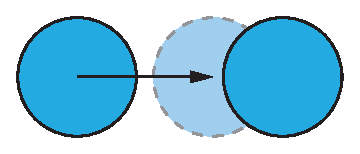
\includegraphics[width=0.4\textwidth]{kolizjatylna.eps}
\caption{Schemat kolizji czołowej, opracowanie własne}
\end{figure}
